\documentclass[12pt]{article}
\usepackage[margin=0.5in,top=0.5in,bottom=0.5in]{geometry}
\usepackage{amsmath}
\usepackage{indentfirst}
\usepackage{scrextend}
\usepackage{graphicx}
\graphicspath{{images/}}

\title{\textbf{\underline{Assignment 1 Report}}}
\author{Anoop (2015CS10265)}

\begin{document}
\pagenumbering{gobble}
\maketitle

\section*{\underline{Linear Regression}}
\subsection*{Part a}
\begin{addmargin}[0.3in]{0in}
Learning Rate ($\eta$) - 0.0015 \\
Stopping criteria - $cost\ <\ 0.0001$ or $iterations\ >\ 101$ \\
Final Parameters - $\theta_0 = 0.9966201$ and $\theta_1 = 0.0013402$
\end{addmargin}
\subsection*{Part b}
\begin{center}
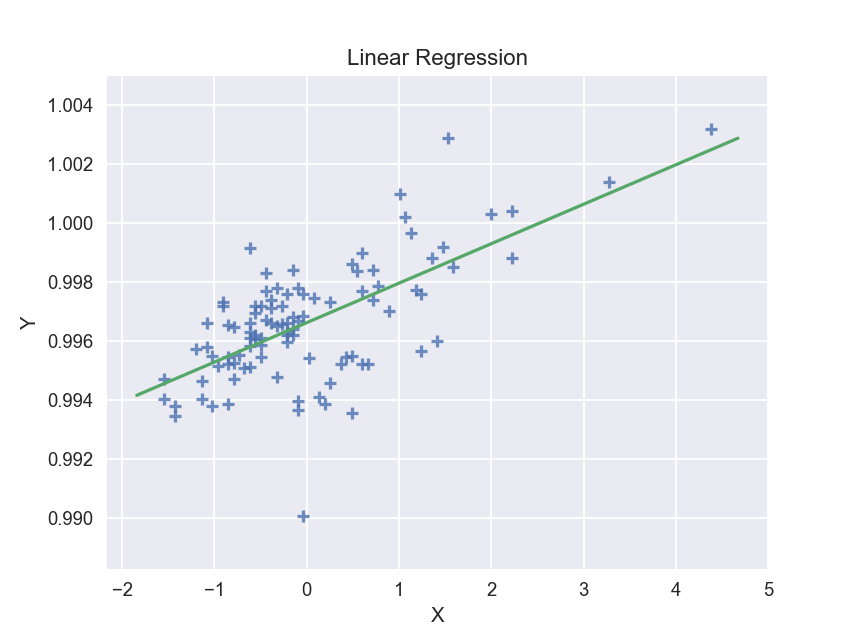
\includegraphics[scale=0.5]{linear1.png}
\end{center}
\subsection*{Part c}
\begin{center}
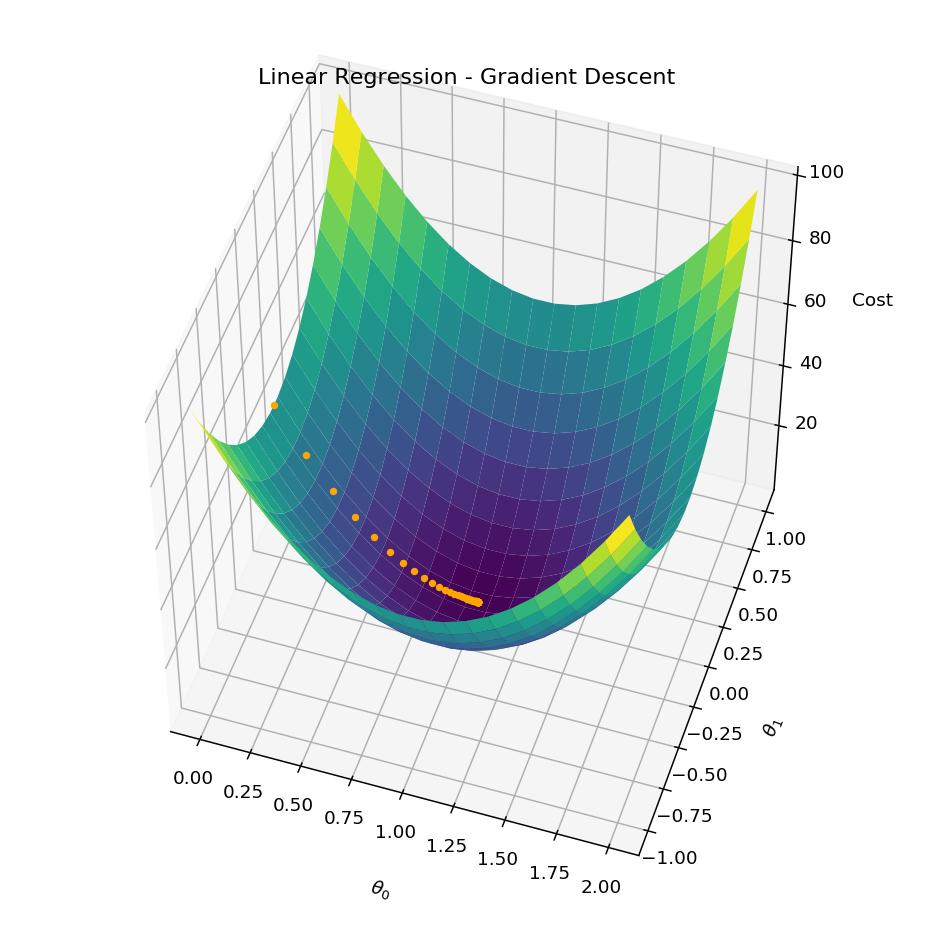
\includegraphics[scale=0.35]{linear2.png}
\end{center}
\subsection*{Part d}
\begin{center}
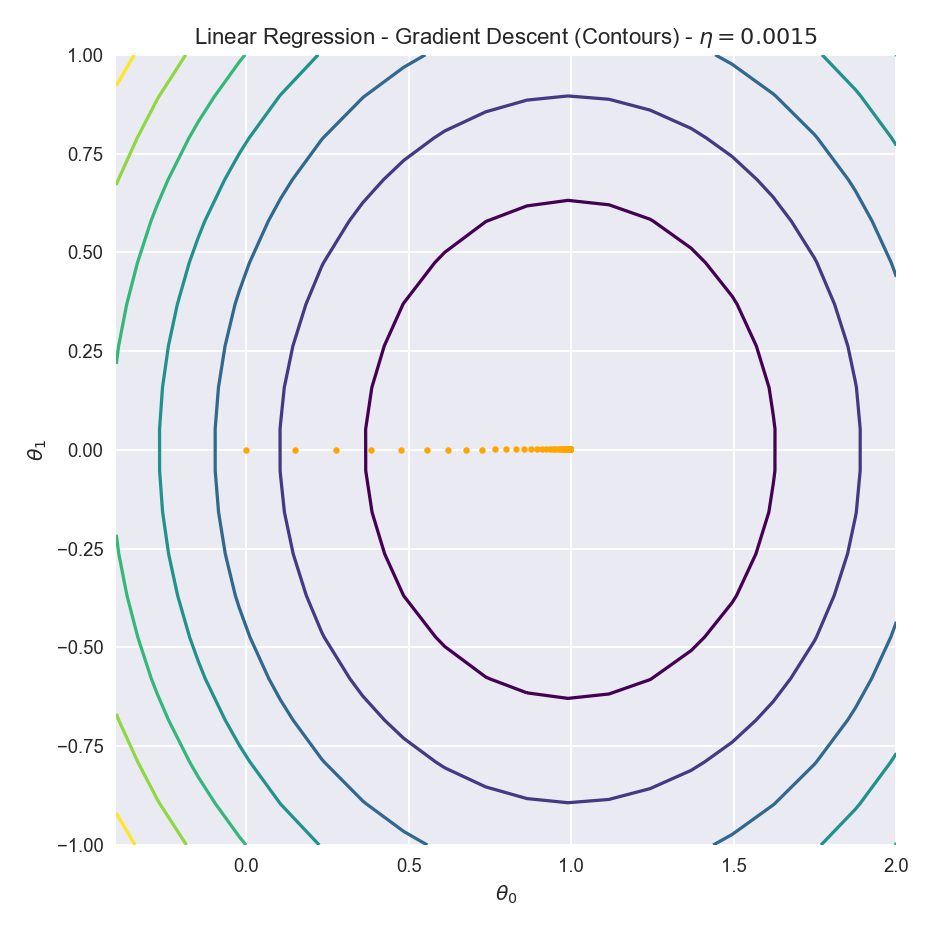
\includegraphics[scale=0.35]{linear3.png}
\end{center}
\subsection*{Part e}
\begin{figure}[!htb]
\begin{tabular}{cc}
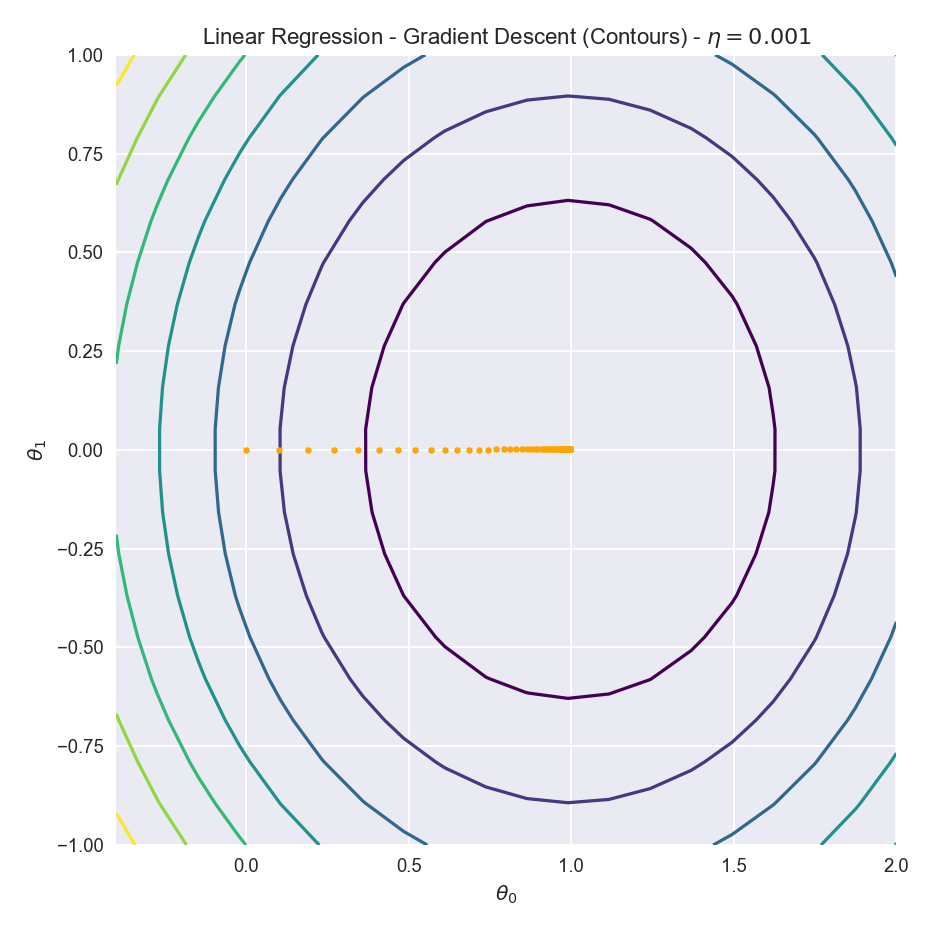
\includegraphics[scale=0.3]{linear4.png} & 
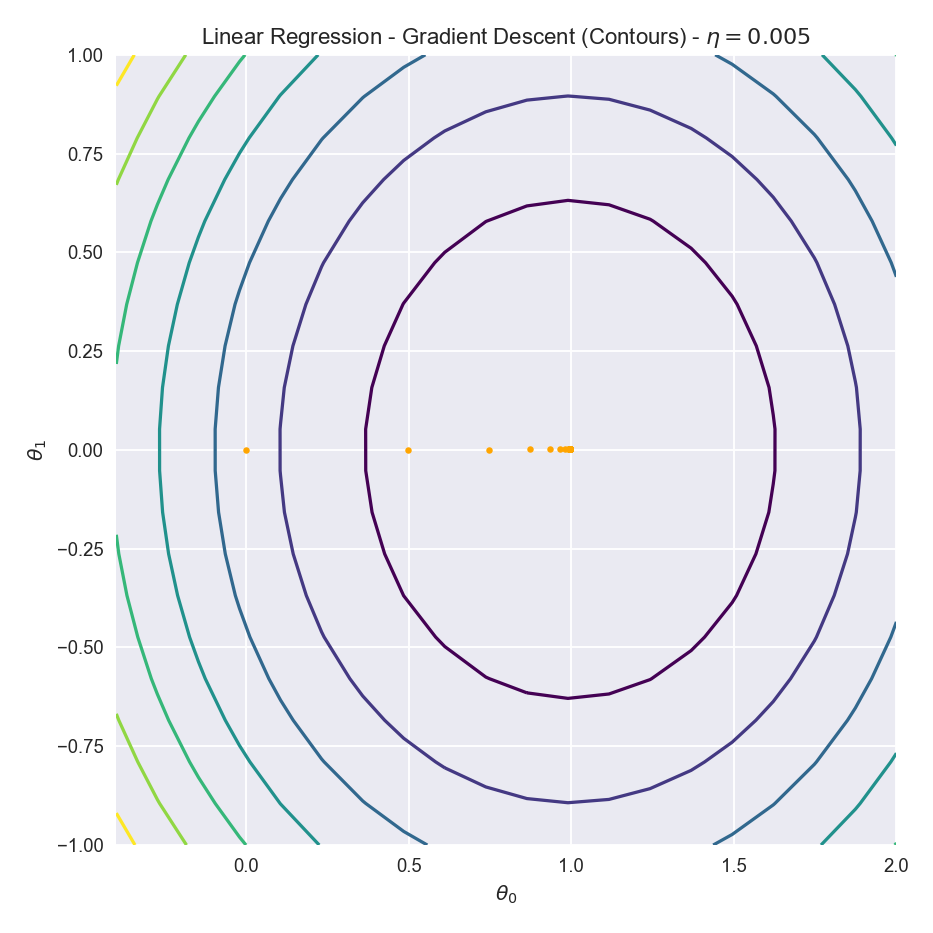
\includegraphics[scale=0.3]{linear5.png} \\
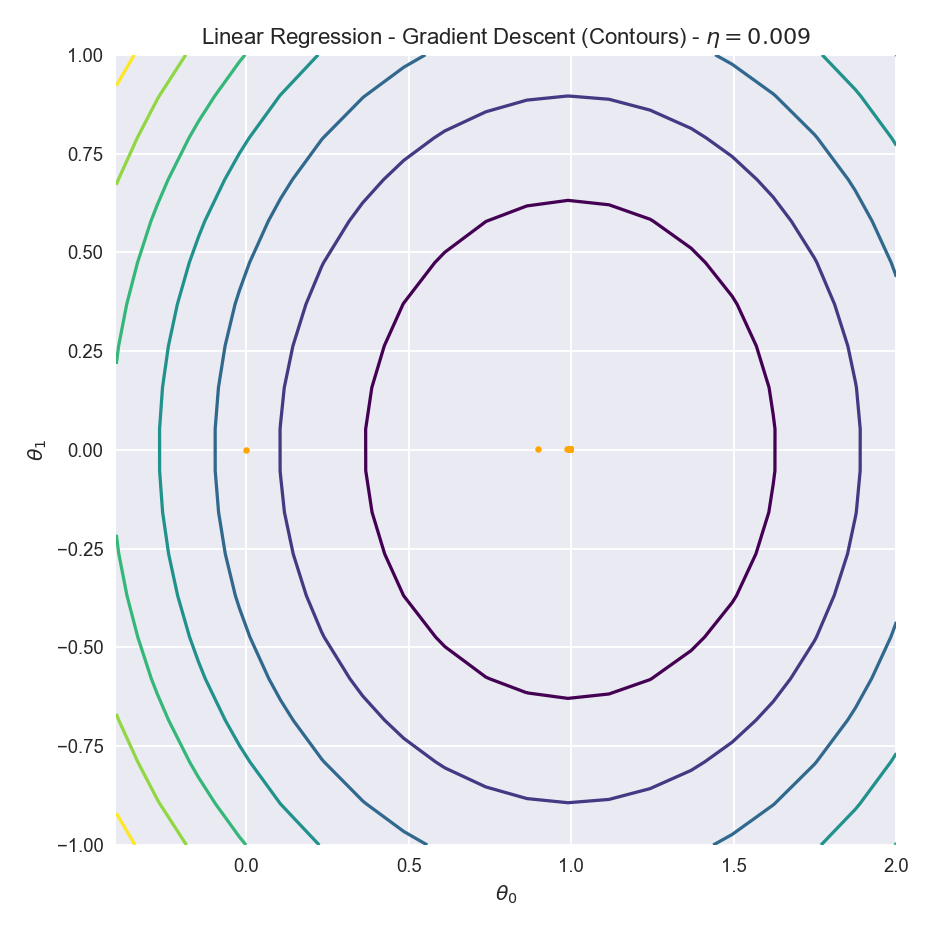
\includegraphics[scale=0.3]{linear6.png} & 
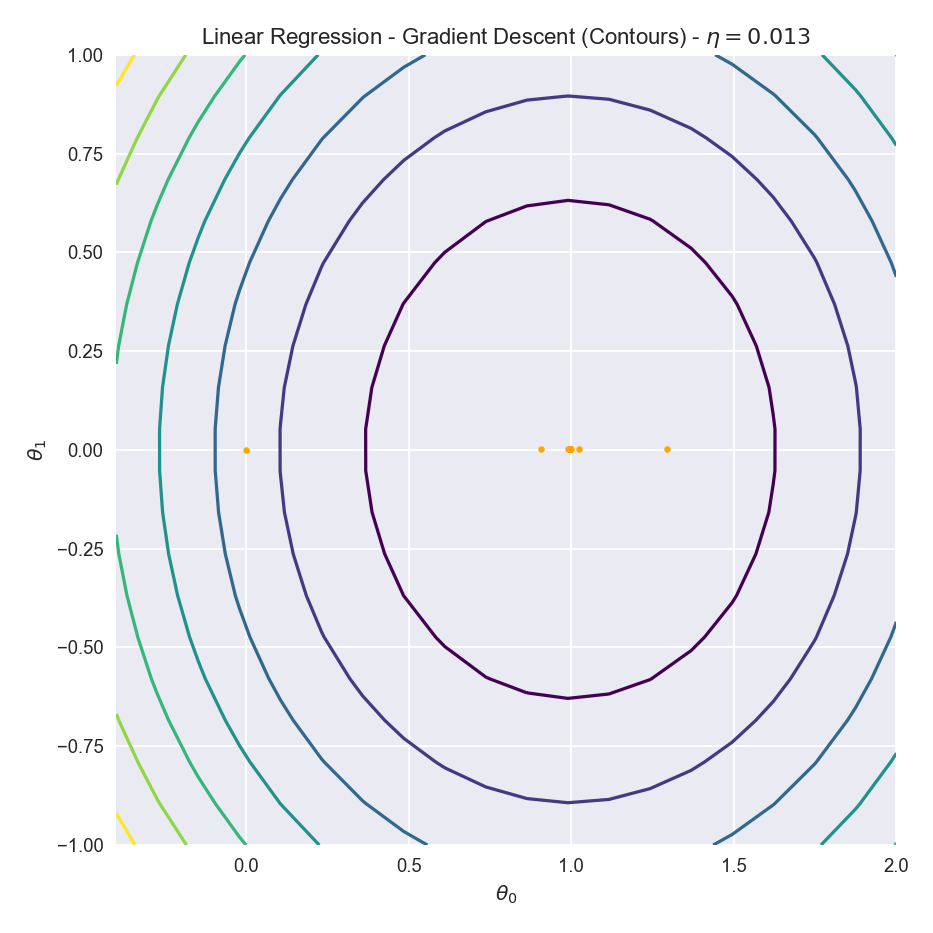
\includegraphics[scale=0.3]{linear7.png} \\
\end{tabular}
\end{figure}
\newpage
\begin{figure}[!htb]
\begin{tabular}{cc}
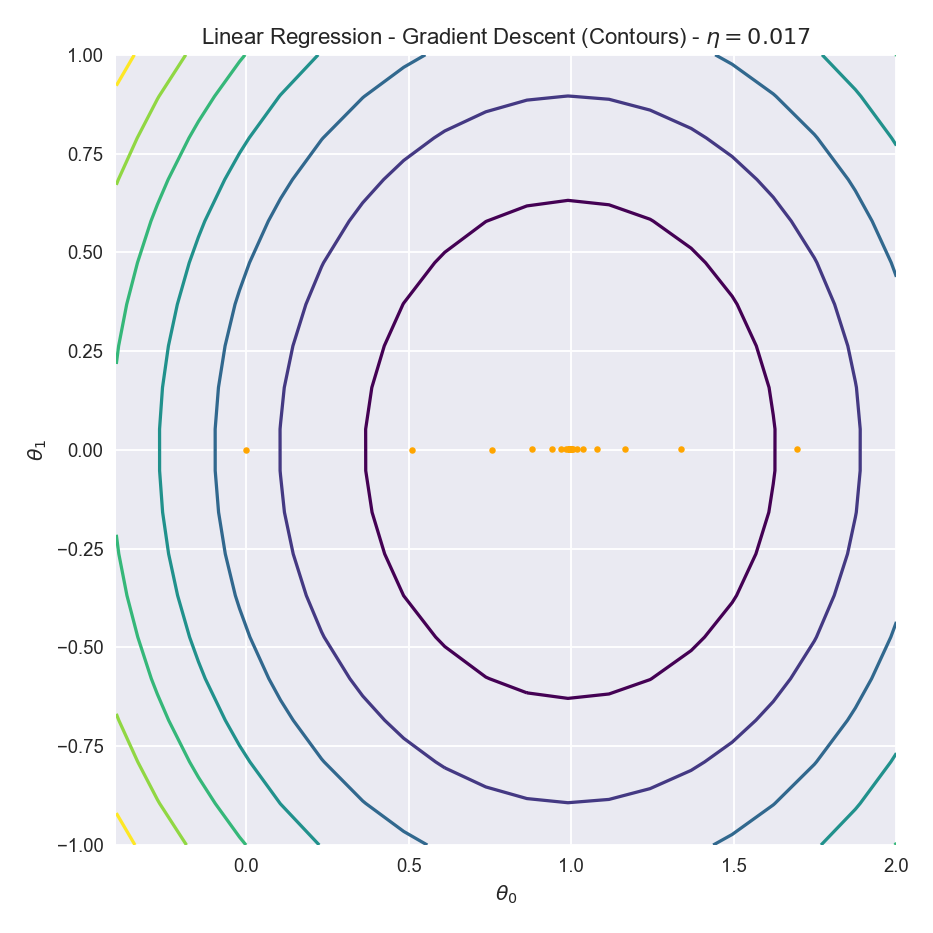
\includegraphics[scale=0.3]{linear8.png} & 
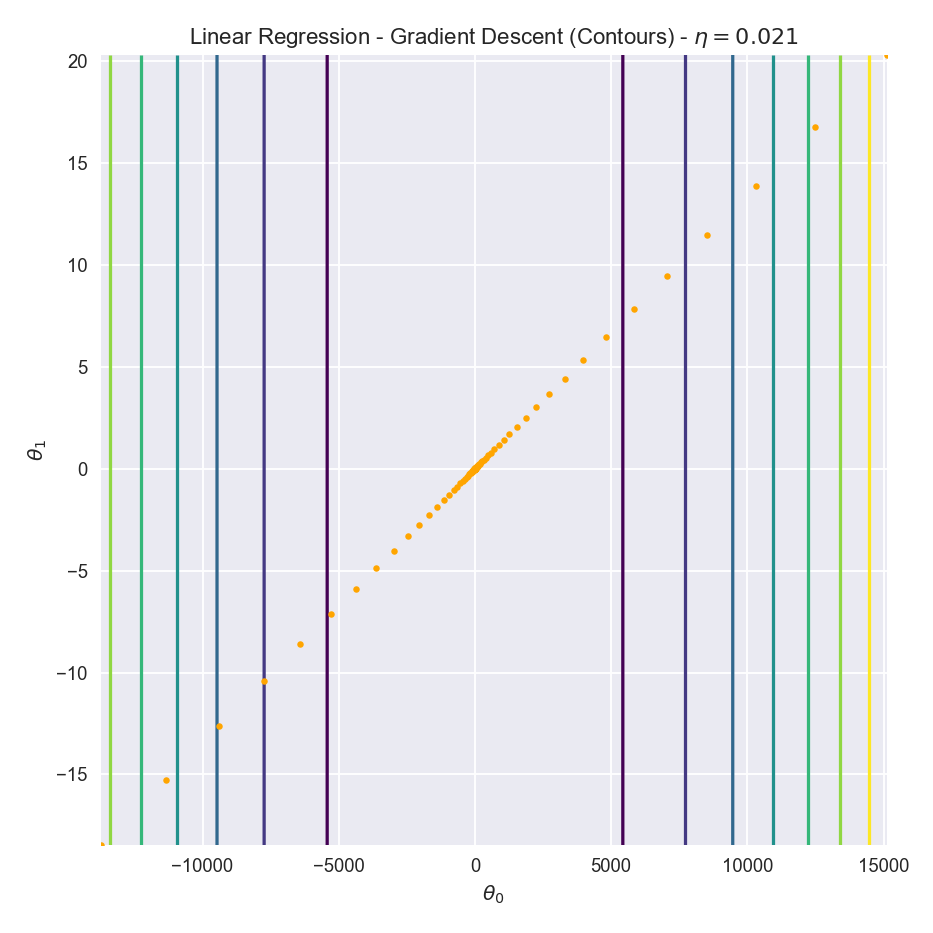
\includegraphics[scale=0.3]{linear9.png} \\
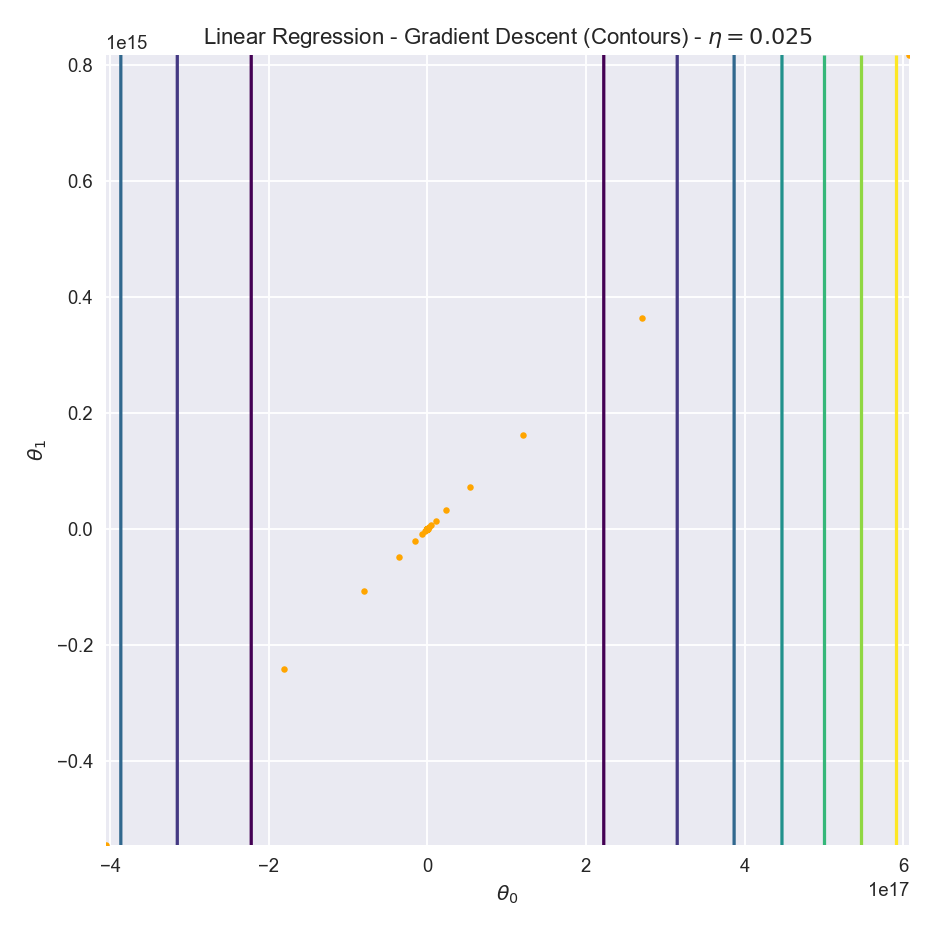
\includegraphics[scale=0.3]{linear10.png}
\end{tabular}
\end{figure}
\begin{addmargin}[0.3in]{0in}
From the contours for various learning rates, it is clear that as the learning rate increases beyond some point, the cost function starts diverging. After initial overshooting, there are large oscillations around the minimum, each time overshooting even more.
\end{addmargin}

\newpage
\section*{\underline{Locally Weighted Linear Regression}}
\subsection*{Part a}
\begin{addmargin}[0.3in]{0in}
Final Parameters - $\theta_0 = 1.03128116$ and $\theta_1 = 0.83519315$
\end{addmargin}
\begin{center}
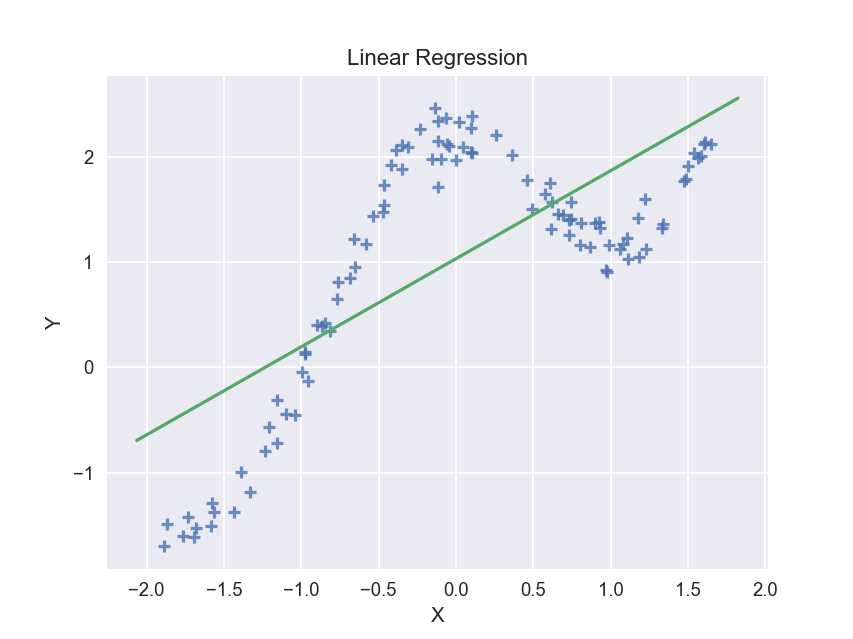
\includegraphics[scale=0.45]{localweight1.png}
\end{center}
\subsection*{Part b}
\begin{center}
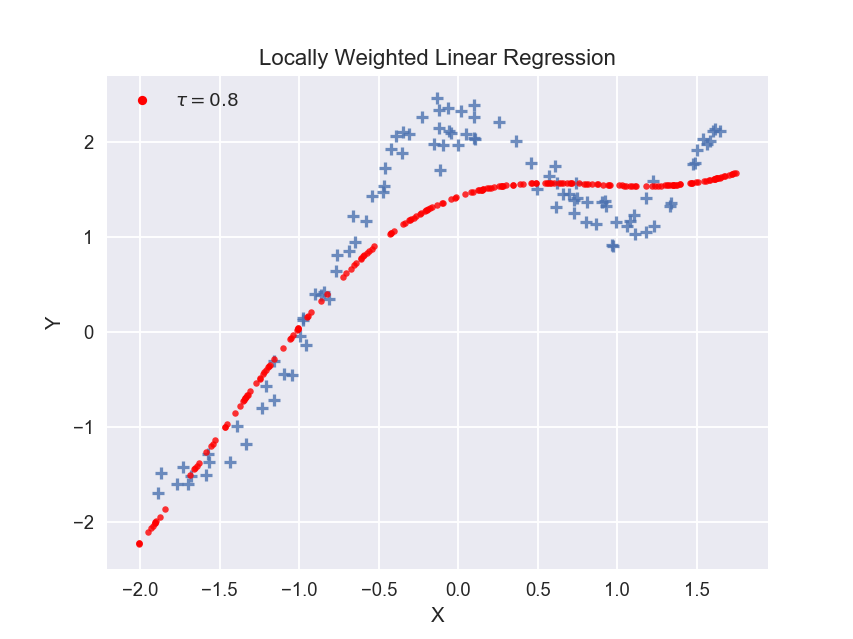
\includegraphics[scale=0.45]{localweight2.png}
\end{center}
\subsection*{Part c}
\begin{center}
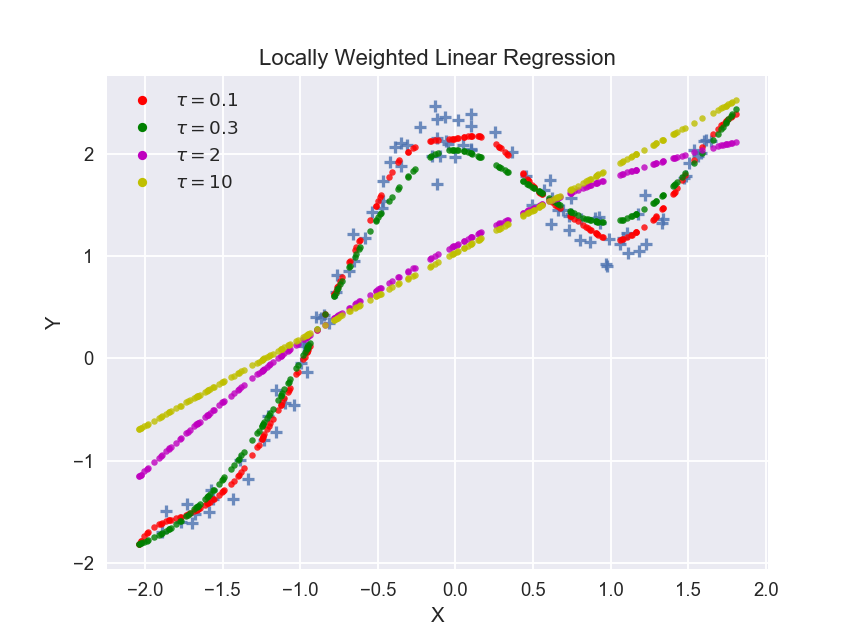
\includegraphics[scale=0.4]{localweight3.png}
\end{center}
\begin{addmargin}[0.3in]{0in}
As $\tau$ becomes too large, the model starts underfitting (tends to be linear). As $\tau$ becomes too small, the model starts overfitting (tends to pass through all points).
\end{addmargin}

\section*{\underline{Logistic Regression}}
\subsection*{Part a}
\begin{addmargin}[0.3in]{0in}
Final Parameters - $\theta_0 = -0.2130308$, $\theta_1 = -2.65801937$ and $\theta_2 = 2.66106075$
\end{addmargin}
\subsection*{Part b}
\begin{center}
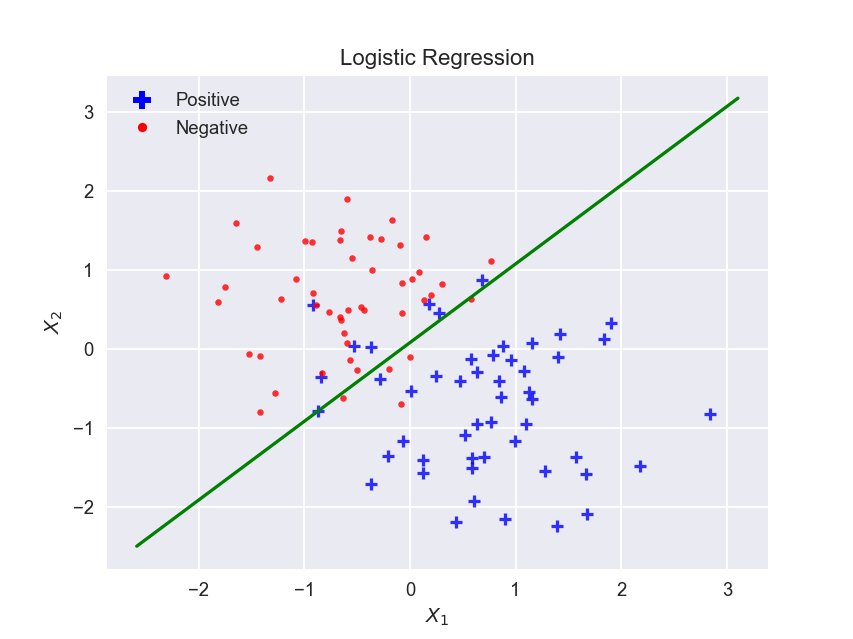
\includegraphics[scale=0.4]{logistic1.png}
\end{center}

\newpage
\section*{\underline{Gaussian Discriminant Analysis}}
\subsection*{Part a}
\begin{addmargin}[0.3in]{0in}
$\mu_0 = \begin{bmatrix} 137.46 & 366.62\end{bmatrix}^{T}$ \\
$\mu_1 = \begin{bmatrix} 98.38 & 429.66\end{bmatrix}^{T}$ \\
$\Sigma_0 = \Sigma_1 = \Sigma = 
\begin{bmatrix}
    287.482 &  -26.748 \\
    -26.748 & 1123.25
\end{bmatrix}$
\end{addmargin}
\subsection*{Part b}
\begin{center}
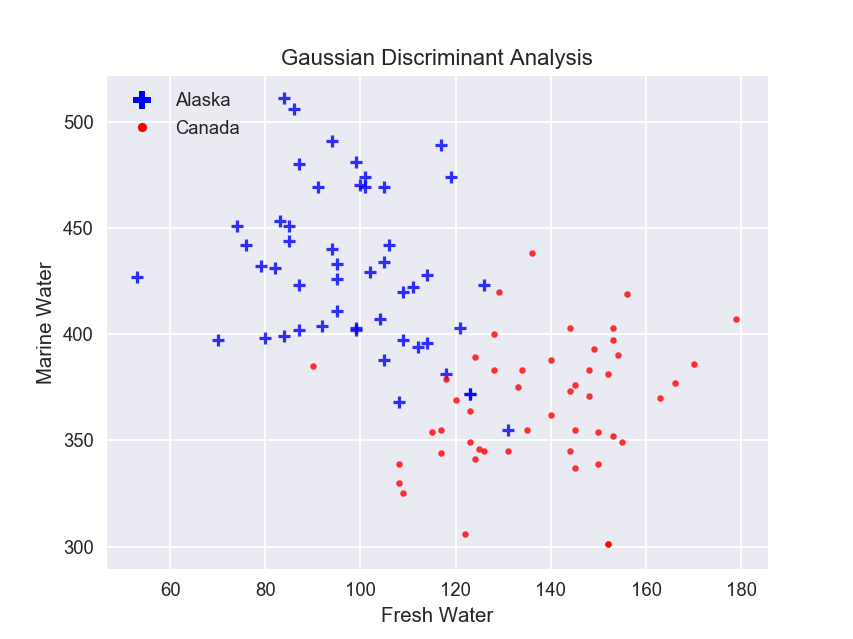
\includegraphics[scale=0.4]{gda1.png}
\end{center}
\subsection*{Part c}
\begin{center}
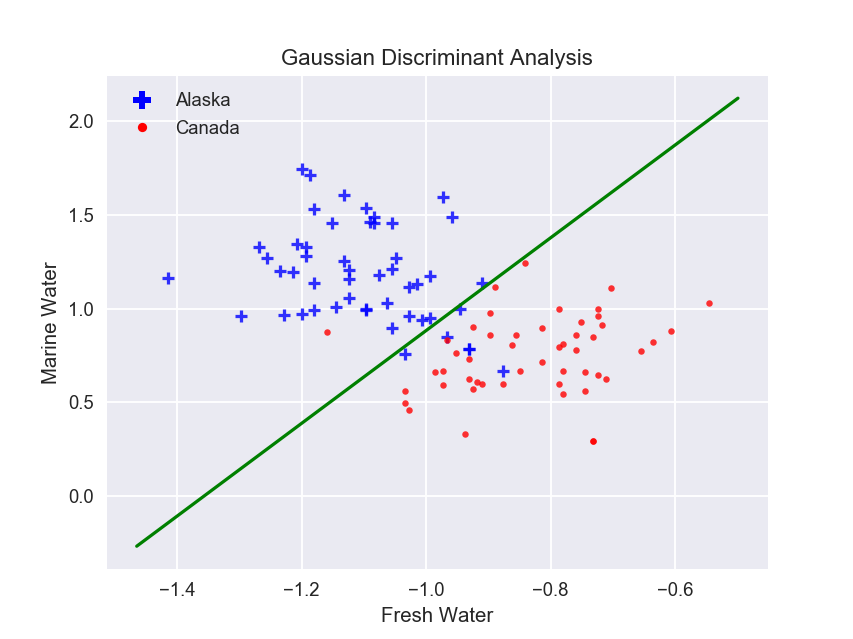
\includegraphics[scale=0.4]{gda2.png}
\end{center}
\subsection*{Part d}
\begin{addmargin}[0.3in]{0in}
$\mu_0 = \begin{bmatrix} 137.46 & 366.62\end{bmatrix}^{T}$ \\
$\mu_1 = \begin{bmatrix} 98.38 & 429.66\end{bmatrix}^{T}$ \\
$\Sigma_0 = 
\begin{bmatrix}
    319.5684 & 130.8348 \\
    130.8348 & 875.3956
\end{bmatrix}$ \\
$\Sigma_1 = 
\begin{bmatrix}
    255.3956 & -184.3308 \\
    -184.3308 & 1371.1044
\end{bmatrix}$
\end{addmargin}
\subsection*{Part e}
\begin{center}
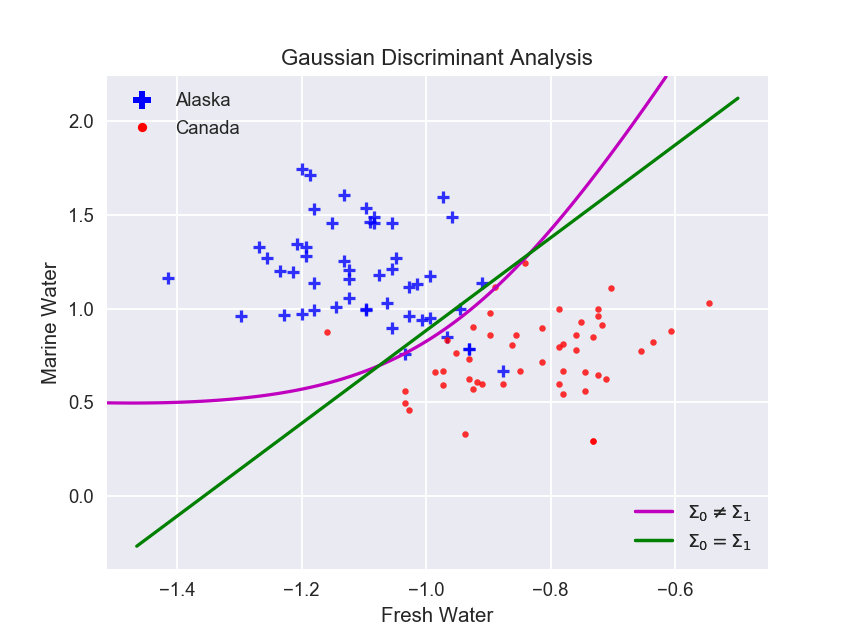
\includegraphics[scale=0.5]{gda3.png}
\end{center}
\subsection*{Part f}
\begin{addmargin}[0.3in]{0in}
From the plot (in Part e) we can see that the quadratic decision boundary does better job of classification than the linear decision boundary (equivalent to logistic regression). This means that the assumption that the underlying data belongs to Gaussian distribution is valid to a great extent.
\end{addmargin}

\end{document}